\newpage
\chapter{Optimising the inDrop Single-Cell RNA-seq Platform}
\label{ch:indrop}

\section{Redesigning inDrop}
\label{sec:redesigning_indrop}
As shown in chapter \ref{ch:litrev}, droplet microfluidics have been applied extensively in high-throughput single-cell technology. Single cells are co-encapsulated with various reagents and barcoded hydrogel beads in order to capture their nucleic acid content (figure \ref{fig:indrop_scrna_overview}). The first part of this thesis revolves around the optimisation of inDrop, a leading droplet microfluidic single-cell \acrshort{rna-seq} technique \citep{klein2015}. We implemented a number of changes to the original inDrop protocol, most of which were inspired by other droplet microfluidic protocols such as Drop-seq and 10x Genomics' commercial \acrshort{scrna-seq} solution. First, we physically altered the microfluidic protocol to improve quality of life and ease of operation. Next, we changed the reverse transcription reaction and library preparation steps to a \acrshort{smart-seq} approach. An overview of the major changes is given in figure \ref{fig:indrop_compar_combo}.\pms

% The main goal of these changes was to improve ease of handling and price of the inDrop protocol while retaining or increasing the quality of the resulting data.
%
\begin{figure}[ht]
\centerfloat
\includegraphics[width=\textwidth]{./ims/indrop_scrna_overview.png}
\caption[General overview of an inDrop experiment]{\textbf{General overview of an inDrop experiment.} Single cells are encapsulated into a nanolitre volume droplet together with a barcoded hydrogel bead. The cell is lysed, and its \acrshort{mrna} content is tagged in a reverse transcription reaction using the hydrogel's barcoded primers. The \acrshort{cdna} libraries of thousands of cells are then pooled and processed for sequencing.}
 \label{fig:indrop_scrna_overview}
\end{figure}

\clearpage
\begin{figure}[ht]
\centerfloat
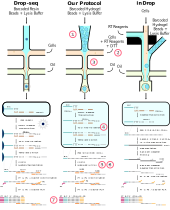
\includegraphics[width=17cm]{./ims/indrop_compar_combo.png}
\caption[Molecular changes to the inDrop protocol]{\textbf{Molecular changes to the inDrop protocol.} Red markers indicate major differences or improvements.}
 \label{fig:indrop_compar_combo}
\end{figure}

\clearpage
\begin{enumerate}
	\item We retained inDrop's soft, deformable hydrogel beads in order to keep the super-Poissonian bead loading, but scaled them down to a smaller size (\SI{50}{\micro\metre} instead of \SI{70}{\micro\metre}). With this change in size, we aimed to produce beads compatible with the 10x Chromium microfluidic chips.
	\item inDrop beads release their primers into the cell droplet by cleavage of a \acrshort{uv}-sensitive linker. We replaced this linker with a disulfide bond which can be cleaved by \acrshort{dtt}-mediated reduction in the droplet. This change greatly improves handling of beads during all steps of the process as they do not need to be shielded from ambient light any more.
	\item inDrop employs a system of 3 input flows - one each for cells, hydrogel beads and \acrshort{rt}/lysis reagents. While such a setup allows for fine control over all flows, it complicates microfluidic operation. We adopted Drop-seq's microfluidic design by merging lysis buffer flow with bead flow and \acrshort{rt} reagent flow with cell flow.
	\item Like Drop-seq, we opt for a \acrshort{smart-seq}-like template-switching reverse transcription which incorporates a \acrfull{tso} at the 3' end of the \acrshort{cdna} transcripts. In our case, the \acrshort{tso} bears a sequence complementary to the 5' end of the barcode. Template switching thus induces end-complementarity into the transcript which will play an important role in step 5. The template-switching reverse-transcription reaction takes place \textit{in} the droplet, as opposed to Drop-seq's pooled \acrfull{stamp} approach.
	\item We bypass inDrop's time-consuming \acrlong{ivt} based amplification protocol by using \acrfull{ispcr}. \acrshort{ispcr} employs a single primer which hybridises to both ends of the \acrshort{cdna} transcript. Short fragments form hairpins, obstructing primer hybridisation and thus amplification, reducing classical \acrshort{pcr} bias towards shorter fragments.
	\item We replace inDrop's random hexamer \acrlong{rt} library prep with the off-the-shelf NEBNext ligation protocol. This approach is very similar to Drop-seq's classic Nextera library preparation, which uses Tn5 tagmentation and adapter \acrshort{pcr}. NEB and NXT indicate the NEB and Nextera adapters.
	%\item Both Drop-seq and inDrop use a combination of enzymatic digestion digestion and several size-selective bead purification steps to filter out leftover primers throughout various parts of their respective workflows. In our protocol, we rely on size-selective bead purification only in order to reduce time to sequencing.
	\item Whereas inDrop sequences the cell barcode in one dedicated sequencing read on the Illumina \acrshort{ngs} platforms, our cell barcode is read in two separate reads. We thereby avoid sequencing the fixed sequence in-between both barcode halves and dedicate these sequencing cycles to the \acrshort{cdna} instead. This will be detailed in chapter \ref{ch:seq}.
\end{enumerate}

The result of these changes is a more streamlined protocol for high-throughput droplet-microfluidic single-cell \acrshort{rna-seq}.\pms

\clearpage

\begin{figure}[ht]
\centerfloat
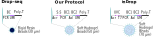
\includegraphics[width=\textwidth]{./ims/indrop_beads.png}
\caption[Differences in bead and barcode structure]{\textbf{Hydrogel bead barcode structure.} For Drop-seq - \acrshort{pcr}: \acrshort{pcr} primer site, BC: barcode, \acrshort{umi}: unique molecular identifier. For our protocol and inDrop - Acr: Acrydite linker, S-S: disulfide bond \acrshort{pcr}: priming site for isothermal amplification during barcoding, BC1 and BC2: both halves of the barcode used in split-pool barcode generation, Ad: \acrshort{pcr} adapter used in split-pool barcode generation, T7: T7 promoter used in in-vitro transcription. UVC: inDrop's UV-Cleavable spacer.}
 \label{fig:}
\end{figure}

\subsection{Methodology and Work Plan}
We systematically set up and streamlined our inDrop workflow according to a set plan illustrated in figure \ref{fig:indrop_workplan}. First, we produced a standardised stock of barcoded hydrogel beads to use during all following experiments. We then performed a number of dry inDrop runs to find the right flow rates for optimal bead and cell loading. Next, we progressed onto "true" inDrop runs with high concentrations of cells. These runs were progressed up to the library preparation stage. We performed several intermediate quality control steps on these sequencing libraries, such as \acrshort{dna} quantification and fragment length distribution analysis, and made adequate changes to the library preparation protocols. Finally, we performed a complete inDrop run that was sequenced on the Illumina NextSeq 500 platform. The resulting data is shown and analysed in chapter \ref{ch:seq}.

\begin{figure}[ht]
\centerfloat
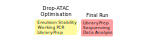
\includegraphics[width=\textwidth]{./ims/indrop_workplan.png}
\caption[inDrop workplan]{\textbf{inDrop workplan.}}
\label{fig:indrop_workplan}
\end{figure}

\newpage
\section{Manufacturing Barcoded Hydrogel Beads}
\label{sec:indrop_bhbproduction}
Both the \acrshort{scrna-seq} method described this chapter and the \acrshort{scatac-seq} method of chapter \ref{ch:dropatac} will make extensive use of hydrogel beads. These hydrogel spheres serve as carriers for the barcoded oligonucleotide payload used to index a cell's nucleic acid material. Because inDrop hydrogels are soft and deformable, they can be loaded into microfluidic channel at high concentrations, leading to a stacking effect that allows for near-deterministic control of hydrogel flow. Such a highly-controllable flow essentially removes a large amount of stochasticity from the cell encapsulation process, leading to more efficient sample loading and lower cost \citep{klein2015, abate2009}. This section describes the general workflow for the production of these hydrogel beads, as well as a deterministic model for estimating the microfluidic parameters required for a given hydrogel diameter.\pms

\subsection{Hydrogel Bead Production}
\label{subsect:indrop_beadproduction}
First, hydrogel beads carrying short \acrshort{dna} stubs are produced using standard polyacrylamide chemistry adapted for microdroplet generation on a microfluidic chip \citep{zilionis2017}. These chips are produced according to standard protocols described in \ref{app:meth_mfchips}. A flow of mixed monomer/crosslinker/acrydite oligo is emulsified into monodisperse droplets in fluorinated oil. The fluorinated oil phase contains \acrshort{temed}, which catalyses the polymerisation reaction by accelerating free radical formation from \acrshort{aps}. The resulting emulsion is incubated overnight at \SI{65}{\celsius} during which the individual monomer droplets polymerise into spherical hydrogels. After extensively washing to remove all traces of apolar solvents and unused reagents, the hydrogel beads are ready for barcoding. The detailed protocol is described in \ref{app:meth_beadgen}. Figure \ref{fig:indrop_beadgen} shows the dimensions of the microfluidic chip and the polymerisation reaction involved in the process.\pms

\begin{figure}[ht]
\centerfloat
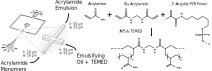
\includegraphics[width=\textwidth]{./ims/indrop_beadgen2.png}
\caption[Hydrogel bead generation chip and chemistry]{\textbf{Hydrogel bead generation chip and chemistry.}}
 \label{fig:indrop_beadgen}
\end{figure}

\subsection{Modelling Hydrogel Bead Diameter}
\label{subsect:indrop_model}

\begin{wrapfigure}{R}{\textwidth/3+6pt}
\vspace{-10pt}
\centering
\includegraphics[width=\textwidth/3]{./ims/indrop_beads_emulsion.png}
\captionsetup{margin={6pt,6pt},labelfont=bf}
\caption[Hydrogel emulsion before polymerisation]{\textbf{Hydrogel emulsion before polymerisation.}}
\label{fig:indrop_beads_emulsion}
\vspace{-30pt}
\end{wrapfigure}

The diameter of the hydrogel beads can be tuned within a range of 30-\SI{80}{\micro\metre} by adjusting the flow rates of oil ($Q_{oil}$) and monomer/crosslinker ($Q_{oil}$) during droplet generation. The size of the hydrogel beads directly determines the amount of barcoded primer they can carry, which impacts the efficiency of reverse transcription (for inDrop) or \acrshort{pcr} (for drop-\acrshort{atac}). Moreover, loading only hydrogels of controlled size and shape into the microfluidic device will facilitate microfluidic operation, preventing non-linear behaviour such as shockwaves and oscillations. Having a monodisperse distribution of diameter size is thus crucial for our application. We chose a set bead diameter of \SI{50}{\um}, which is similar in size to 10x's hydrogel beads. Having a similar bead diameter would allow us to benchmark the beads without accounting for variability in microfluidic operation. Additionally, such beads could be used to develop new protocols for the 10x Chromium, which is more user-friendly than in-house microfluidic setups.\pms

As the diameter of the beads increases by up to 25\% during polymerisation and subsequent washing steps, predicting bead diameter based on emulsion droplet diameter is difficult. In order to find the flow parameter settings that would produce monodisperse beads of \SI{50}{\micro\metre}, we formulated a model that can predict the diameter of the final beads based on the flow rates used during bead generation. We used an experimental design approach to maximise the amount of information we could extract from the labour and costs associated with producing the hydrogel beads. We designed a blocked response surface experiment with 2 blocks of 4 combinations according to the methodology described in \cite{goos2011}. We proposed a quadratic model as they are a relatively simple class of models and often sufficiently explain variation in a process. Observations were blocked by the microfluidic chip used to account for variation between individual chips. During the experiments, it became apparent that 2 of the 8 combinations did not produce any droplets, but instead resulted in laminar oil and monomer co-flows. This occurred when the ratio of monomer to oil flow was greater than \textasciitilde{}1.5. We therefore augmented the initial design with two additional blocks of each 3 runs constrained to oil/monomer > 1.5, for a total of 12 samples (\ref{app:meth_beadgen}).\pms

In order rapidly and efficiently measure bead diameter, a Python image analysis script was written which could batch analyse a number of microscopy images from the beads. The script uses the \verb|opencv| library to fit circular objects within set distances from each other, and automatically returns their diameters and locations within the frame. Figure \ref{fig:indrop_algorithm} shows an example of the script's accuracy. The script itself can be found in \ref{app:supp_python}.\pms

\begin{figure}[ht]
\centerfloat
\includegraphics[width=103.91795mm]{./ims/indrop_algorithm.png}
\caption[Bead diameter script example]{\textbf{Bead diameter script example.} Arrow indicates a bead that went undetected by the image analysis script.}
 \label{fig:indrop_algorithm}
\end{figure}

We then produced the 12 batches of beads according to the parameters dictated by our experimental design and measured them after all washing steps were completed. The resulting dataset comprised \textasciitilde{}8000 beads unequally divided over the 12 parameter combinations, shown in supplementary figure \ref{fig:indrop_model_data} (sample 16 was omitted, as it was a statistical outlier and located at the edge of what physically resulted in beads). Based on this dataset, two separate models were estimated - one relating flow rates and bead diameter (eq. \ref{eq:beaddiam}), and the second relating flow rates and the \textit{variation on} bead diameter (eq. \ref{eq:beadvar}). As bead diameter was (by design) heteroscedastic over the parameter space and our dataset was heavily imbalanced, we used \acrfull{reml} to estimate the diameter model parameters (\ref{app:meth_model}). We then used mixed stepwise regression control to iteratively select significant effects (p < 0.05). Heredity was invoked for $Q_{oil}$ as it occurs in significant interaction effects. Units are \si{\micro\metre} and \si[per-mode=symbol]{\micro\litre\per\hour} for diameter and flow respectively:\pms

\begin{equation}
\label{eq:beaddiam}
	\begin{aligned}
	% d = 53.55717041 - 12.6127716*10^{-3} Q_{mono} - 568.748135*10^{-3} Q_{oil} - 3.431768*10^{-6} Q_{mono} Q_{oil} + 11.11989482*10^{-6} Q_{mono}^{2} - 612.288979*10^{-9} Q_{oil}^{2}
	d = \SI{53.6}{\um} & - \num{12.6e-3} \SI[per-mode=fraction]{}{\um\hour\per\ul}\times Q_{mono} - \num{569e-3} \SI[per-mode=fraction]{}{\um\hour\per\ul}\times Q_{oil}\\
	& - \num{3.43e-6} \SI[per-mode=fraction]{}{\um\hour\squared\per\ul\squared}	\times Q_{mono}\times Q_{oil}\\
	& + \num{11.1e-6} \SI[per-mode=fraction]{}{\um\hour\squared\per\ul\squared}	\times Q_{mono}^{2} - \num{612e-9} \SI[per-mode=fraction]{}{\um\hour\squared\per\ul\squared} \times Q_{oil}^{2}
	\end{aligned}
\tagaddtext{[\si{\micro\metre}]}
\end{equation}

\begin{equation}
\label{eq:beadvar}
	\begin{aligned}
	% \sigma_{d} = 3.8357659353 + 996.2582*10^-6 Q_{mono} - 1.61705107*10^-3 Q_{oil} - 256.4131265*10^-9 Q_{mono} Q_{oil}
	\sigma_{d} = \SI{3.84}{\um} & + \num{996e-9} \SI[per-mode=fraction]{}{\um\hour\per\ul} \times Q_{mono} - \num{1.62e-3} \SI[per-mode=fraction]{}{\um\hour\per\ul} \times Q_{oil}\\
	& - \num{256e-9} \SI[per-mode=fraction]{}{\um\hour\squared\per\ul\squared}
	\times Q_{mono}\times Q_{oil}\\
	\end{aligned}
\tagaddtext{[\si{\micro\metre}]}
\end{equation}

Equation \ref{eq:beaddiam} was then set to \SI{50}{\micro\metre} and used as a constraint on flow rates in a non-linear minimisation of equation \ref{eq:beadvar}. This resulted in a set of flow rates that will yield a predicted diameter of \SI{50}{\micro\metre} at the lowest possible diameter variation. The entire modelling process is visualised in fig. \ref{fig:indrop_model} and \verb|MATLAB| code can be found in \ref{app:supp_matlab}.\pms

\begin{figure}[ht]
\centerfloat
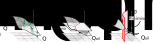
\includegraphics[width=\textwidth]{./ims/indrop_model.png}
\caption[Bead parameter modelling]{\textbf{Bead parameter modelling.} A surface response is fitted through diameter data gathered on the experimental design flow parameters. Diameter is then fixed to the desired amount, and the intersection is used as a constraint space in a minimisation problem on the second model, which relates standard deviation and flow.}
\label{fig:indrop_model}
\end{figure}

% \begin{wrapfigure}{L}{\textwidth/3+6pt}
% \vspace{-10pt}
% \centering
% \includegraphics[width=\textwidth/3]{./ims/indrop_beads_polymerised.png}
% \captionsetup{margin={6pt,6pt},labelfont=bf}
% \caption[Hydrogel beads after polymerisation]{\textbf{Hydrogel beads after polymerisation.}}
% \label{fig:indrop_beads_emulsion}
% \vspace{-30pt}
% \end{wrapfigure}
%
For our desired diameter of \SI{50}{\micro\metre}, the models suggested flows of \SI[per-mode=symbol]{1461}{\micro\litre\per\hour} and \SI[per-mode=symbol]{1500}{\micro\litre\per\hour} for $Q_{oil}$ and $Q_{mono}$ respectively. Using these parameter combinations, we produced a batch of hydrogel beads which will be used throughout this thesis. These hydrogels averaged a diameter of \SI{53}{\micro\metre} with a standard deviation of \SI{5}{\micro\metre}, which was sufficiently close to the target diameter for us to continue to the barcoding step. As producing hydrogels takes 2-3 work days, we did not further validate the model for other diameters. The model will be reused (and validated) on new microfluidic chips to produce beads of different diameters in the near future, when we may require beads of a different size for different protocols.

% When we wanted to reuse the microfluidic chips from the first run after 5 months, we made an interesting observation. Our old parameter settings (1500 and \SI[per-mode=symbol]{1461}{\ul\per\hour}) did not produce beads of the desired size anymore. During this prolonged time spent in storage, a thin layer of viscous oil had formed inside the chip's channels. This thin film significantly altered the diameter of the channels and thus flow characteristics of chip. We suspect the film is formed after evaporation of \acrshort{hfe} used for surface treatment. \pms

\clearpage
\subsection{Barcoding the Beads}
\label{subsect:indrop_barcoding}
In order to equip every single hydrogel bead with clonal copies of a pseudo-unique barcode, we performed two sequential split/pool reactions according to \cite{zilionis2017}, giving each bead in the stock one out of 147 456 possible barcodes. In a stock of millions, the beads are thus not unique ("pseudo-unique"), but in a single experiment using \textasciitilde{100 000} beads, the chance of collisions is low. The barcoding is shown graphically in figure \ref{fig:indrop_splitpool} and the detailed protocol is given in \ref{app:meth_splitpool}.\pms

\begin{figure}[ht]
\centerfloat
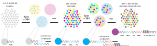
\includegraphics[width=\textwidth]{./ims/indrop_splitpoolv2.png}
\caption[Hydrogel bead barcoding process]{\textbf{Hydrogel bead barcoding process.} Unbarcoded hydrogel beads are split into 384 wells where a first well-specific, barcoded primer hybridises to the acrydite stub via a \acrshort{pcr} handle (PCR). Barcode 1 (BC1) is then appended to the acrydite stub by isothermal amplification. The beads are re-pooled and re-split in 384 new wells where a second well-specific barcode (BC2) is appended to the first via an adapter sequence (Ad). This adapter sequence will also serve as a sequencing primer site later on. The split/pool process leads to 384 x 384 = 147 456 possible paths that a bead may have travelled, and thus an equal number of barcode combinations. Adapted from \cite{zilionis2017}}
 \label{fig:indrop_splitpool}
\end{figure}

We then performed two simple quality control experiments on the \acrfullpl{bhb}. First, we performed a series of \acrshort{fish}-like experiments during different stages of the barcoding process to asses if the previous step had succeeded (figure \ref{fig:indrop_beadqcv2}). After every step in the barcoding process, beads that had just undergone isothermal amplification were incubated with a fluorescent \acrshort{fam} probe complementary to the newly appended barcode part. As a negative control, beads that did not undergo the last step were also incubated with the fluorescent probe. The results of these tests were as expected - only those beads that had undergone barcoding showed a fluorescent signal. A background signal is detected in \ref{fig:indrop_beadqcv2}-b, which could be explained by the change in camera setup or non-specific binding. Theoretically, it is possible to quantify the light intensity signal from the beads to estimate the amount of primer on the oligo. We did not apply this method as our camera setup was not fixed, but plan to do this once a fixed camera epifluorescence microscope is available.\pms

\begin{figure}[ht]
\centerfloat
\includegraphics[width=\textwidth]{./ims/indrop_beadqcv2.png}
\caption[BHB FISH quality control]{\textbf{\acrshort{bhb} \acrshort{fish} quality control.} (Un)barcoded hydrogel beads were incubated with a fluorescent \acrshort{fam} probe, washed, and examined under a microscope. The following combinations were used: a) unbarcoded beads with an acrydite stub \acrshort{pcr}  primer probe, b \& c) unbarcoded and partially barcoded beads with an adapter probe, d \& e) partially and fully barcoded beads with a poly-A probe.}
 \label{fig:indrop_beadqcv2}
\end{figure}

Second, we tested whether the disulfide-cleavage mediated release of primers from the beads worked as planned. Here, beads were incubated in various concentrations of \acrshort{dtt}, after which the presence of released oligo in the supernatant was detected using \acrshort{qpcr} (\ref{app:meth_qpcr}). The concentration of beads was equal to the ratio of bead to water inside the droplet during an inDrop run. The resulting data showed that there is no significant difference between the amount of primers released by \SI{10}{\milli\molar} or \SI{125}{\milli\molar} of \acrshort{dtt} (figure \ref{fig:indrop_qpcr}).\pms

\begin{figure}[ht]
\centerfloat
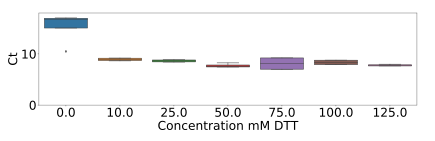
\includegraphics[width=\textwidth]{./ims/indrop_qpcr.png}
\caption[Bead oligo release qPCR results]{\textbf{Bead oligo release qPCR results.}}
\label{fig:indrop_qpcr}
\end{figure}

We therefore continued our experiments with the lowest concentration of \acrshort{dtt} in order to not disturb the reverse transcription reaction. It can be seen that even at \SI{0}{\milli\molar} \acrshort{dtt}, there is a significant concentration of primer in the supernatant. This can be explained by either contamination of the sample - that is, supernatant still containing beads after centrifugation - or contamination of the bead stock with free-floating primers. As these free-floating primers would barcode the cell's nucleic acid without sharing a barcode with that cell's bead oligos, they would negatively impact the specificity of the inDrop \acrshort{scrna-seq} results. As of now, the true impact of possible stock contamination and how to reduce it is unclear.\pms

\begin{wrapfigure}{L}{\textwidth/3+6pt}
\vspace{-10pt}
\centering
\includegraphics[width=\textwidth/3]{./ims/indrop_failed10x_2.png}
\captionsetup{margin={6pt,6pt},labelfont=bf}
\caption[Failed 10x run with custom beads]{\textbf{Failed 10x run with custom beads.} Arrows indicate cells.}
\label{fig:indrop_failed10x}
\vspace{10pt}
\end{wrapfigure}

After sieving them through a \SI{70}{\um} filter, we attempted to use the freshly barcoded beads on the 10x Chromium microfluidic chip as originally intended. We loaded the beads onto the chip as per chip manufacturer's instructions, and started the run. Sadly, the Chromium did not generate droplets with beads in them - a very crude emulsion with large droplets was formed in most output wells instead. The single output well which had formed a monodisperse emulsion, did not contain any beads. This suggests that dust in the bead stock had blocked the chip's fine microchannels before our beads could reach the flow focusing point, resulting in a beadless emulsion (figure \ref{fig:indrop_failed10x}). This dust would go on to become a major hurdle we had to overcome when producing a working microfluidic assay.\pms

\clearpage
\section{Execution of the Improved inDrop Protocol}
\label{sec:improved_indrop}
This section will detail all of the (partial) inDrop runs we performed and the rationale between the specific parameter settings employed.\pms

% \begin{figure}[ht]
% \centerfloat
% \includegraphics[width=\textwidth/3*2]{./ims/indrop_chip_zoom.png}
% \caption[inDrop chip]{\textbf{inDrop chip.}}
% \label{fig:indrop_chip_zoom}
% \end{figure}
%
\subsection{Preliminary Bead and Cell Loading Tests}
First, we wanted to get acquainted with the microfluidic chip. We performed a number of dry trial runs with only beads to explore the flow rate settings that would lead to sufficient bead loading. The cell flow was replaced by mock flow of \acrshort{pbs} at \SI{777}{\ul\per\hour}. During the first run, dust from the bead stock immediately began blocking the fine microfluidic channels (figure \ref{fig:indrop_dust}), halting the entire process and in some cases leading to delamination of the \acrshort{pdms} from the glass slide due to overpressure.\pms

\begin{wrapfigure}{L}{\textwidth/3+6pt}
\vspace{-15pt}
\centering
\includegraphics[width=\textwidth/3]{./ims/indrop_dust.png}
\captionsetup{margin={6pt,6pt},labelfont=bf}
\caption[Dust blocking microfluidic channel]{\textbf{Dust blocking microfluidic channel.}}
\label{fig:indrop_dust}
\vspace{-35pt}
\end{wrapfigure}

We suspect this dust was introduced during the barcoding process, as the 4 96-well reaction plates are exposed to the open air for 10-30 minutes during manual addition of the barcoded primers. After barcoding, the \acrshortpl{bhb} are washed several times and filtered through a \SI{70}{\um} filter. This filtering process was repeated a number of times after the dust was observed, but did not completely eliminate all dust from the stock. The filtering step also leads to small losses, so it was not repeated after two more times.\pms

To solve or alleviate the dust issue, we came up with three possible solutions:

\begin{enumerate}
	\item Eliminate dust from the barcoding process by using an automated liquid handler in an enclosed space. We started working on automated barcoding protocols for the Hamilton Microlab STAR early on, before the first round of barcoding took place. During initial tests, we found that the viscous properties of the bead solution and the low volumes used during barcoding would require careful fine-tuning of the STAR protocol. We therefore barcoded the first batch of beads manually. Automation of the barcoding is an ongoing project.
	\item Filtering the beads by simply running them through an inDrop chip, and switching to a fresh chip when dust blocks the channels. This strategy produced a very pure bead solution, but took an exhausting amount of time at \SI{300}{\ul\per\hour}. Due to high viscosity of the bead stock, higher flow rates would usually lead to delamination problems or produce pressures high enough to push dust through the channels.
	\item Produce a filtering inDrop chip design. In the first filter design, a number of tightly-packed columns blocked both large and small dust filaments from entering the microfluidic channels while allowing beads and cells to pass. In practice, this design often suffered from delamination as the very fine filter acted as a point of high resistance for the bead stock to pass. We therefore adjusted the design with a set of more streamlined filters, which provided a functional balance between filtering capacity and fluid resistance. Figure \ref{fig:indrop_filters} shows the different filter designs.
\end{enumerate}

Out of all options considered, the filtering inDrop chip design yielded the best practical result, so we continued down that path.\pms

\begin{figure}[ht]
\centerfloat

\includegraphics[width=\textwidth]{./ims/indrop_filters.png}
\caption[inDrop Filter Design Evolution]{\textbf{inDrop filter design evolution.}}
\label{fig:indrop_filters}
\end{figure}

\begin{wrapfigure}{L}{\textwidth/3+6pt}
\vspace{-15pt}
\centering
\includegraphics[width=\textwidth/3]{./ims/indrop_coverage.png}
\captionsetup{margin={6pt,6pt},labelfont=bf}
\caption[inDrop dry run bead coverage]{\textbf{inDrop dry run bead coverage.}}
\label{fig:indrop_coverage}
\vspace{-20pt}
\end{wrapfigure}

Once the dust issue was under control, we started fine-tuning the flow rates used for bead/cell encapsulation, starting with beads only (\ref{app:meth_indrop_opt}). After a few rounds of trial and error, we found that flow rates of \SI{300}{\ul\per\hour} for mock cell flow (\acrshort{pbs}), \SI{200}{\ul\per\hour} for beads and \SI{450}{\ul\per\hour} for oil achieved a \textasciitilde{90}\% coverage for beads in droplets. In later runs with cells, we were not able to achieve such high coverages due to low sample volumes not permitting adjustment before the run ended. In the final run that was eventually sequenced, we also used higher average flow rates to increase speed and combat cell sedimentation/sticking to the chip.\pms

We then started performing inDrop runs with beads and cells to try to achieve good droplet coverage of both cells and beads. During these trials, and the next, we used either melanoma (MM087 or MM074) or breast cancer (MCF7) cells, as they were readily available to us in the lab and we were interested in the physical properties of the system rather than the biological properties of the cells. The \acrshort{rt} enzyme was replaced by an equal volume of 50\% glycerol to reduce cost and retain the flow properties of the \acrshort{rt} mix. Cells are rapidly lysed after they come into contact with the bead/lysis mix, making it difficult to asses how well the cells have loaded. As we were still in the process of setting up the protocol in pilot runs, we decided to keep cell concentrations high during all experiments described in this thesis (initially up to \SI[per-mode=symbol]{800000}{\per\ml}, gradually scaled down to \SI[per-mode=symbol]{300000}{\per\ml}) to ensure a signal and to combat cells sticking to the microfluidic chip and tubing. A side-effect of this approach is low per-cell signal after sequencing, as the number of reads is limited per sequencing run. In a true single-cell experiment, we would scale the cell concentration down by a factor 10-100 to increase per-cell sequencing depth.\pms

During these trials, we also found that the cells formed an insoluble precipitate together with the master mix, which again led to complete obstruction of the microfluidic channel. After a number of replacements and additions to the \acrshort{rt} master mix, we succeeded in reducing - but not completely eliminating - cell precipitation. The main change was the removal of \acrshort{bsa} from the cell suspension. \acrshort{bsa} was originally incorporated here to prevent cells from sticking to each other and to the microfluidic tubing. We also tried to pre-incubate the tubes instead of coating the cells with \acrshort{bsa}. This reduced cell-sticking to a minimum, but the film of \acrshort{bsa} delaminated from the tubing when brought into contact with the \acrshort{rt} mix. We therefore removed all \acrshort{bsa} from the protocol, which led to higher cell sticking, but strongly reduced precipitation.\pms

% \todo[inline]{show what we did to solve the precipitation - remove the \acrshort{bsa} from the mix}

\subsection{Generating cDNA Libraries}
After the cell suspension precipitation was reduced, we started performing inDrop runs with beads, cells and functional \acrshort{rt} mix. The emulsions generated here were incubated on a heat block for \acrlong{rt} and, if they passed \acrshort{cdna} quantification on the Qubit, were further processed for \acrshort{ispcr}. Figure \ref{fig:ind_snapshot} shows a still of a single cell about to be encapsulated in the microfluidic chip.\pms

\begin{figure}[ht]
\centerfloat
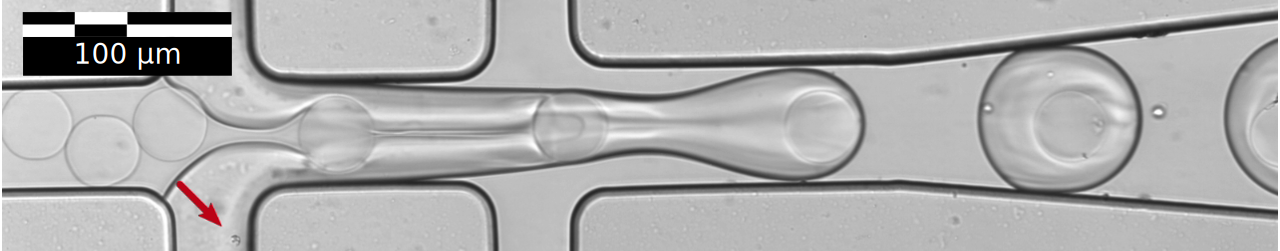
\includegraphics[width=\textwidth]{./ims/ind_snapshot.png}
\caption[inDrop snapshot]{\textbf{inDrop snapshot}. Arrow indicates a cell about to be encapsulated.}
\label{fig:ind_snapshot}
\end{figure}

In the first trial (\ref{app:meth_first_indrop_trial}), we used an \acrshort{rt} master mix containing 11.25\% \acrshort{peg}, which is present for molecular crowding of the \acrshort{rt} reaction, and no \acrshort{bsa}. After reverse transcription, we pooled the libraries by breaking the droplets. Here, we measured \SI{259}{\ng} of \acrshort{dna}. Half of the library was treated with Exo I to remove residual primers left in the sample. Both samples were \acrshort{ispcr}-amplified using Terra polymerase. After a second round of clean-up, including Ampure bead filtering of small fragments, the Exo I treated sample yielded only \SI{12}{\ng} of \acrshort{dna}, and the untreated sample \SI{57}{\ng}. This was deemed insufficient, and we did not process the libraries further.\pms

\begin{wrapfigure}{R}{\textwidth/3}
\centering
\includegraphics[width=\textwidth/3]{./ims/ind_suresh.png}
\captionsetup{margin={6pt,6pt},labelfont=bf}
\caption[Final inDrop run droplets]{\textbf{Final inDrop run droplets.}}
\label{fig:ind_suresh}
\vspace{-20pt}
\end{wrapfigure}

In the second trial (\ref{app:meth_second_indrop_trial}), we wondered if the Terra enzyme may have been at fault, producing such low amount of \acrshort{dna} in the first trial. We therefore decided to exactly repeat the first trial, but process half of the sample with Terra polymerase, and half of the sample using KAPA HiFi polymerase. We did not perform any Exo I treatment, as it seemed to had negatively affected the yield in the previous run. Now, the Terra \acrshort{pcr} run produced \SI{104}{\ng} of \acrshort{dna}, and the Kapa \acrshort{pcr} run produced only \SI{22}{\ng} of \acrshort{dna} after Ampure bead cleanup. However, this library failed the library preparation stage as described in the next section.\pms

The final run that was eventually processed for sequencing was performed by a senior lab scientist, and did not incorporate \acrshort{peg} in the \acrshort{rt} suspension. This run, which was performed on MM087 melanoma cells, passed all quality control stages, and was also successfully processed for sequencing. Figure \ref{fig:ind_suresh} shows the droplets generated in this final run. These droplets were generated at higher flow rates than the previous runs (800, 1100 and \SI{1200}{\ul\per\hour} for cells, beads and oil), as this reduced runtime, meaning less time for the cells to sediment and the enzymes to denature.\pms

\subsection{Library Preparation Troubles}
After we had achieved a sufficient yield after the \acrshort{ispcr} stage, moved on to sequencing library preparation. As we wanted to sequence the libraries using Illumina's sequencing by synthesis technology, we needed to append P5 and P7 adapters to all barcoded fragments. These adapters are used on the Illumina flow cell to generate clusters using bridge amplification. In our case, the P5 adapter comes with a sample index which can be used to demultiplex pooled samples after sequencing.\pms

% \begin{figure}[ht]
% \centerfloat
% \includegraphics[width=\textwidth/2]{./ims/indrop_failednextera.png}
% \caption[Failed Nextera library preparation electropherogram]{\textbf{Failed Nextera library preparation electropherogram.} The fragment distribution is too broad, too long and has an enrichment of small fragments, indicating residual primers.}
% \label{fig:indrop_failednextera}
% \end{figure}

Initially, we planned to perform adapter tagging using a classical Illumina Nextera XT kit, which first tagments the library and appends P5 and P7 adapters to the Tn5 adapters using \acrshort{pcr}. Due to unknown reasons, this library prep approach failed multiple times on our library, producing no or low yields of amplified \acrshort{dna}, and an unfavourable fragment length distribution (figure \ref{fig:supp_nextera}). We therefore tried the NEBNext Ultra II Library Prep Kit, which did produce a sequencing library. This kit works by fragmenting the \acrshort{cdna} and ligating a special hairpin loop adapter to both ends of the fragments. This hairpin is then enzymatically cleaved open to produce non-complementary strand ends which can be used to selectively amplify one strand. The NEBNext kit thus utilises a hairpin loop to produce strand-specific sequencing libraries, which can be used to identify antisense transcripts. These transcripts may play an important role in regulating gene expression \citep{mills2013}. The entire final library preparation process is outlined in figure \ref{fig:indrop_detail} and, together with the inDrop run protocol, in \ref{app:meth_indrop}.\pms

\clearpage
\begin{wrapfigure}{L}{8cm}
\centering
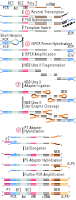
\includegraphics[width=7.65cm]{./ims/indrop_detail.png}
\captionsetup{margin={0pt,0pt},labelfont=bf}
\caption[inDrop sequencing library prepartion]{\textbf{inDrop sequencing library preparation.}}
\label{fig:indrop_detail}
\end{wrapfigure}

1. Barcoded poly-T primers are released into the droplet by the hydrogel bead and hybridise to Poly-A\textsuperscript{+} \acrshort{mrna} from the lysed cell. An \acrshort{mmlv} reverse transcriptase catalyses the reverse transcription and adds a string of cytosine nucleotides to the 3' end of the \acrshort{cdna} transcript which serves as a hybridisation site for the \acrfull{tso}. The \acrshort{tso} is used as a template for further polymerisation by the \acrshort{mmlv} reverse transcriptase and contains the reverse sequence of a \acrshort{pcr} primer that is also present at the 5' end of the barcode, leading to complementarity of both ends.\medskip

2. The single-cell \acrshort{cdna} libraries are then pooled and undergo \acrshort{ispcr}, where we add a single \acrshort{pcr} primer which can hybridise on either of the transcript. Fragments that contain a short \acrshort{cdna} strand can form hairpin loops, preventing hybridisation and thus reducing the size-selective bias associated with classical \acrshort{pcr}.\medskip

3. The \acrshort{cdna} is then fragmented, end-repaired and dA-tailed using the NEB Ultra II Illumina Library prep protocol. The NEB hairpin adapter is then ligated and cleaved, resulting in two non-complementary primers on the sense and antisense strands.\medskip

4. Lastly, the adapter-ligated library is \acrshort{pcr}-amplified with Illumina P7 and P5 adapters. First, a P7-\acrshort{pcr}-primer hybridises to the 3' end of the antisense strand, and elongation occurs. Only now, the i5-P5-\acrshort{pcr}-primer hybridisation site is present, and exponential amplification can occur. This \acrshort{pcr} is thus selective for the antisense \acrshort{cdna} strand of the barcoded fragment.\medskip
\clearpage

\subsection{Sequencing Results}
\begin{wrapfigure}{L}{\textwidth/2}
\centering
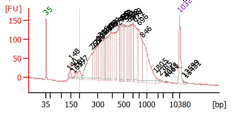
\includegraphics[width=\textwidth/2]{./ims/indrop_C3_bioanalyzer.png}
\captionsetup{margin={6pt,6pt},labelfont=bf}
\caption[inDrop electropherogram]{\textbf{inDrop electropherogram.}}
\label{fig:indrop_bioanalyzer}
\vspace{-20pt}
\end{wrapfigure}

The final library preparation led us to a library that had an average fragment size of 400 bp as indicated by the Bioanalyzer electropherogram (figure \ref{fig:indrop_bioanalyzer}). This library was sequenced on the Illumina NextSeq 500. The resulting sequencing data was mapped using \acrshort{star}, leading to a 56\% mapping percentage, which is relatively low. We were pleased to see that the library showed a classical \acrshort{rna-seq} profile characterised by exon/transcript agreement and enrichment for transcripts mapping to housekeeping genes. The library was also strongly 3' enriched, showing that our library preparation succeeded in selectively amplifying the barcoded transcript ends only (figure \ref{fig:indrop_genebody_combo}).\pms

% \begin{wrapfigure}{R}{\textwidth/2}
% \centering
% 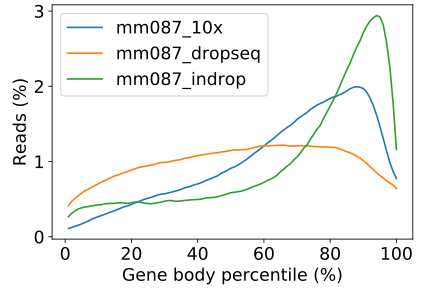
\includegraphics[width=\textwidth/2]{./ims/indrop_genebody.png}
% \captionsetup{margin={6pt,6pt},labelfont=bf}
% \caption[Gene body coverage comparison]{\textbf{Gene body coverage comparison.}}
% \label{fig:indrop_genebody}
% \end{wrapfigure}

\begin{figure}[ht]
\centerfloat
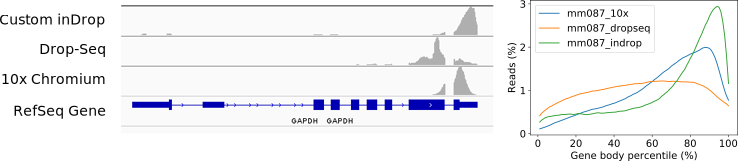
\includegraphics[width=\textwidth]{./ims/indrop_genebody_combo.png}
\caption[Gene coverage comparison]{\textbf{Gene coverage comparison.} Gene coverage of our custom inDrop library is compared to a Drop-seq and 10x Chromium \acrshort{scrna-seq} dataset on the same MM087 cell line. GAPDH is a housekeeping gene and used as a reference point. Data are scaled to account for sequencing depth.}
\label{fig:indrop_genebody_combo}
\end{figure}

However, we quickly discovered that the cell barcode could not be retrieved for the vast majority of transcripts. It appeared that only the \acrshort{cdna}, but not the barcodes, had been sequenced well on the Illumina platform. The lack of cell barcodes had effectively turned our single-cell dataset into a (very expensive) bulk \acrshort{rna-seq}. The ramifications of this discovery and how we attempted to explain it will be further detailed in chapter \ref{ch:seq}.\pms


